\documentclass[../../../../main.tex]{subfiles}
\begin{document}

\begin{flushright}
\footnotesize\textit{【自動文字起こし・要確認】}
\end{flushright}

[解] $\triangle ABC$に余弦定理を用いて
\begin{align*}
&b^2 = a^2+c^2-ac \\
\therefore \quad &(b+a+c)(b-a+c) = ac
\end{align*}

\begin{center}
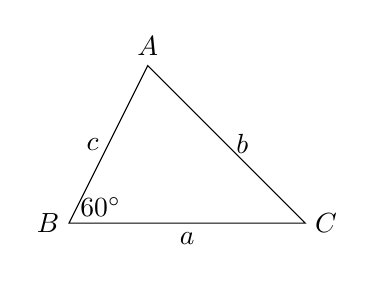
\begin{tikzpicture}[scale=1]
\draw (0,0) node[left]{$B$} -- (3,0) node[right]{$C$} node[midway, below]{$a$} -- (1,2) node[above]{$A$} node[midway, right]{$b$} -- cycle node[midway, left]{$c$};
\node at (0.4, 0.2) {$60^\circ$};
\end{tikzpicture}
\end{center}

$a, c$は素数で、$a \le c$から
$$ (b+a+c, b-a+c) = (a, c) \cdots \text{①}, \quad (1, ac) \cdots \text{②} $$
$$ (b \in \mathbb{Z}, a, c \in \text{素数}, a \le c \text{とする}) $$
である。

①の時
$a=b=c$ となり $\triangle ABC$ は正三角形

②の時
$b = 1-a+c = ac+a-c$ だから $b$を消して
$$ (a-2)(c+2) + 3 = 0 $$
だが、$a, c \in \text{素数}$から$a, c \ge 2$なので、
$$ (\text{正数}) = 0 $$
となり不適。

以上から$\triangle ABC$は正三角形である。

\end{document}
